% ==============================================
% 電気・情報関係学会北陸支部連合大会
% 講演論文投稿用 pLaTeX2e 版テンプレートファイル(2段組)
% Usage: platex jhes2022_platex_utf8_template.tex
% ==============================================
\documentclass[a4paper,10pt]{jarticle}
\usepackage[dvipdfmx]{graphicx}
\usepackage{hyperref}  % もしくは \usepackage{url}
\usepackage{breakurl}  % 長いURLの自動改行
\hypersetup{breaklinks=true}  % hyperrefパッケージのオプション設定
\usepackage{amsmath}
%\usepackage{amsfonts,latexsym}

% ==============================================
% page format
%  textwidth  = paperwidth(210mm) -oddsidemargin(13mm) -evensidemargin(13mm)
%  textheight = paperheight(297mm) -topmargin(20mm-header分) -bottommargin(18mm)
% ==============================================
  \setlength{\paperwidth}{210mm}
  \setlength{\textwidth}{\paperwidth}
  \addtolength{\textwidth}{-13mm} % oddside margin
  \addtolength{\textwidth}{-13mm} % evenside margin
  \setlength{\oddsidemargin}{-1in}
  \addtolength{\oddsidemargin}{13mm} %%%% ここで左右を調節
%
  \setlength{\paperheight}{297mm}
  \setlength{\textheight}{\paperheight}
  \addtolength{\textheight}{-28mm} % 文章領域の高さの調整
  \setlength{\topmargin}{-15mm}    % ここで上下位置を調節
%
  \setlength{\headheight}{0in}
  \setlength{\headsep}{0in}
  \setlength{\columnsep}{10mm}

\makeatletter
\renewcommand{\section}{\@startsection{section}{1}{\z@}%
   {1.5\Cvs \@plus.5\Cvs \@minus.2\Cvs}%
   {.5\Cvs \@plus.3\Cvs}%\and
   {\reset@font\large\bfseries}}   %section見出しの文字サイズをlargeに変更
\renewcommand{\subsection}{\@startsection{subsection}{2}{\z@}%
   {1.5\Cvs \@plus.5\Cvs \@minus.2\Cvs}%
   {.5\Cvs \@plus.3\Cvs}%
   {\reset@font\normalsize\bfseries}} %subsectoin見出しの文字サイズをnormalsizeに変更
   
\makeatother

  \pagestyle{empty}

\begin{document}
\twocolumn[% -- 1段組にしたい場合は,ここをコメントアウトする
% ==============================================
% ページヘッダ(変更禁止)
% ==============================================
%
\begin{center}
{\Large 2024年度電気・情報関係学会北陸支部連合大会}\\
\vspace{-2mm}\rule{\textwidth}{1mm}
\end{center}
% ==============================================
% 原稿はここから
% ==============================================
%
% 講演題目 =====================================
\hspace*{33mm} 
\begin{minipage}{125mm}  %210mm-13mm-13mm-33mm-33mm
\begin{center}    %左づめの場合はflushleft
{\Large \bf
C2Cドックレスシェアサイクル実現に向けた \\
数理最適化ベースの自転車割り当てモデルの構築
}
\end{center}
\end{minipage}
%

\vspace*{4mm}	% ここで行間を調整
%
% 著者名(所属) =====================================
\hspace*{33.0mm} %講演番号用空欄
\begin{minipage}{118mm}  %210mm-13mm-13mm-33mm-33mm
\begin{center}    %左づめの場合はflushleft
{\large
{風折 晃輝(福井大学大学院工学研究科)}

{小高 知宏・松田 優也・黒岩 丈介(福井大学大学院工学研究科)}

{諏訪 いずみ(仁愛女子短期大学)}
}
\end{center}
\end{minipage}

\vspace*{6mm}	% ここで行間を調整
] % -- 1段組にしたい場合は,ここをコメントアウトする


% 本文 =====================================

%\noindent

% section 1 ----
\section{はじめに}
\vspace{-3mm}
\par 欧米やアジアを中心に,自転車を好きなタイミングで好きな期間利用することができるシェアサイクルサービスが世界的に普及している\scalebox{0.7}{\cite{近況}}.しかし,個人が所有している自転車はシェアリングの対象になっていない.あらゆる地域に散在している個人所有の自転車をモビリティのリソースとして有効活用できれば,交通手段の多様化と効率化が促進され,環境負荷の軽減や都市交通の改善にも寄与できるのではないだろうか.そこで,個人所有の自転車を個人間で効率的にシェアリングするため,数理最適化ベースで自転車の割り当てモデルを構築する.

\vspace{-5mm}

% section 2 ----
\section{数理最適化ベースの自転車割り当てモデル}
\vspace{-3mm}
\par 個人所有の自転車をシェアリングの対象とし,ユーザ体験の観点からドックレスで乗り捨て可能なシステムを前提とする.なお,乗り捨てによる自転車の不法駐輪等の法的な課題に関してはここでは考慮せず,あくまで自転車の割り当て問題として切り分けてモデリングする.
\par ユーザリクエストの集合を$J$,シェアリングされる自転車の集合を$B$,ユーザ$j(j \in J)$に自転車$b(b \in B)$が割り当てられたか否かの二値変数行列を$x_{b,j}$,割り当て移動後の距離行列を$d_{b,j}$とする.目的関数は(1)式のように定義し,集合$J$の全てのユーザが移動した後の自転車の散らばりを最小化し,より多くのユーザに自転車を割り当てることを目指す.ただし,$\alpha$は$x_{b,j}$に対する重みである.

\vspace{-8mm}

\begin{flushright}
\begin{equation}
\min \left( \sum_{b}\sum_{j}d_{b,j}x_{b,j} - \alpha\sum_{b}\sum_{j}x_{b,j} \right) \tag{1}
\end{equation}
\end{flushright}

\vspace{-5mm}

% section 3 ----
\section{NYCタクシーデータを用いたシミュレート}
\vspace{-3mm}
\par 構築したモデルを評価・検証するため,C2Cドックレスシェアサイクルの需要に最も親和性が高いと考えられるタクシーの利用データを用いてシミュレーションを行う.シミュレーションに用いるタクシーデータはニューヨーク市(NYC)のタクシー・リムジン委員会(TLC)から提供されている2023年1月のNYCのイエロータクシーのトリップデータ\scalebox{0.7}{\cite{YellowTaxiTripRecords}}を使用することとする.可能な限りドックレスであるシステムの実現を目指すため,ユーザからのリクエストは1分ごとの集合$J$として集約し,(1)式にて定義したモデルに入力し,その他定式化した制約条件のもと割り当て処理を実行する.また,自転車はNYCの主要な約250ポイントのうち,ランダムに10ポイント選択して配置する.
\par 評価方法については,結果として出力される二値変数行列$x_{b,j}$や自転車のステータスを保持する$B$などを元に行う.

\vspace{-5mm}

% section 4 ----
\section{結果と考察}
\vspace{-3mm}
\par 2023年1月1日の24時間のトリップデータを連続的にモデルに入力し,結果的にユーザからのリクエストに対して自転車を割り当てることができた割合と,その際に既に利用中の自転車がどれくらいの割合であったかを示す占有率,サービス提供後に自転車を再配置するためのリバランスコストを図\ref{fig:resultFig}に表す.自転車の占有率は50\%を超えていることが多く,より多くの自転車をユーザに割り当てることができている.一方で,ユーザリクエストに対する割り当て成功率はほとんどの場合で10\%にも満たない.
結果より,NYCに対してランダムに配置している自転車の数が10台で,圧倒的に不足している点が割り当て成功率が極端に低く推移している原因と考えられる.

\begin{figure}[b]
  \centering
  \vspace{-5mm}  % 図の前のスペースを減らす
  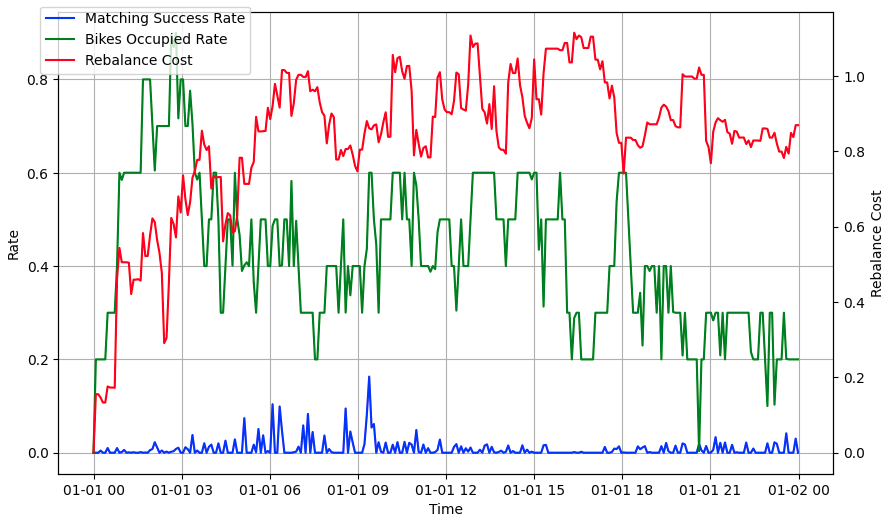
\includegraphics[scale=0.27]
  {figures/dispatchedResultFor1Day.png}
  \vspace{-5mm}
  \caption{自転車の割り当て成功率とステータスの変化}
  \label{fig:resultFig}
  \vspace{-5mm}  % 図の後のスペースを減らす
\end{figure}

\vspace{-5mm}

% section 5 ----
\section{まとめと今後の展望}
\vspace{-3mm}
C2Cドックレスシェアサイクルのための自転車割り当てモデルを構築し,実際のNYCのタクシーデータに基づきリクエストに対して自転車をユーザに割り当てることができた.今後はユーザ体験とシステム効率性のトレードオフを探る点が課題となる.

\vspace{-5mm}

\bibliographystyle{junsrt}
\bibliography{sannkou.bib}
% ==============================================
% 原稿はここまで
% ==============================================
\end{document}
